\documentclass[runningheads]{llncs}
\usepackage{graphicx}
\usepackage{amsmath}
\usepackage{hyperref}

\title{Non-Invasive and Indirect measurement of low sugar concentrations in liquid with the use of ultrasonic sensor}
\titlerunning{Ultrasonic Sensing of Low Sugar Concentrations}

\author{Madhvi Asthana}
\institute{Brandenburg University of Technology, Cottbus-Senftenberg, Germany}

\begin{document}
\maketitle

\begin{abstract}

A capacitive micromachined ultrasonic transducers (CMUT) based sugar concentration detection technique is presented in this work. We know that diabetes is a widely spread disease among adults and over 537 million adults are suffering from it \cite{citation1}. Regular monitoring is very crucial for old-age people, since diabetes may have an effect on the heart and kidneys, which could be a health hazard. Traditional methods like finger-prick blood tests are invasive, painful and expensive for a life-long disease like diabetes.There is a demand for non-invasive, pain-free methods that can be used not only by those diagnosed with diabetes but also by individuals who may be unaware they have the condition. Ultrasonic sensors such as piezoelectric micromachined ultrasonic transducers (PMUT) and capacitive micromachined ultrasonic transducers (CMUT) can be an alternative.
\vspace{1em}  % adds vertical space (~line break)

In the paper we are focusing on CMUT sensor due to its stability in manufacturing, ensuring consistent performance, high sensitivity due to its better receiving strength, RoHS (restriction of hazardous substances in electrical and electronic equipment) compliance, as there is no dangerous material used in CMUT like lead (pb) \cite{citation3}.
\vspace{1em}  % adds vertical space (~line break)

Our experimental results demonstrate that it is possible to estimate sugar concentration at the level significantly below 1\% using a CMUT transducer, which outperforms the state-of-the-art.
\keywords{Ultrasonic sensors \and CMUT \and Non-invasive sugar detection}
\end{abstract}

\section{Introduction}
Detection of subtle sugar concentration is very important in many industries such as food \& beverage, medical \& healthcare industry, fermentation \& brewing industry. Typically, ultrasonic sensors enable estimation of the sugar concentration in a liquid with resolution 2--10\%, which can limit non-invasive quantification of subtle sugar concentration (1 \% or below). 
\vspace{1em}  % adds vertical space (~line break)

Usually, diabetic patients use painful and invasive devices such as accu-chek to monitor their sugar levels- that uses the principle of electrochemical properties. With advancement of technology, minimally invasive techniques are also being explored such as micro-needle, glucowatch, and continuous glucose monitoring device (CGM) which are minimally invasive and less painful. With regard to non-invasive techniques, many technologies have been explored, such as optical techniques like Near-infrared, Raman spectroscopy, Bio-impedence based techniques but they have few shortcomings which may limit their capabilities in terms of accuracy in measurement for example, Raman spectroscopy is very expensive and our one of the goal is to make a method which is inexpensive. Additionally, Bio-impedence or electromagnetic based methods needs high complex signal pre-processing also in such cases tissue conductivity is subjective to change. A system has to be designed which can overcome the shortcoming of earlier researches. 
\vspace{1em}  % adds vertical space (~line break)

Ultrasound is a trusted procedure in medical industry, It's been there in the industry for years. Micromachined Ultrasonic Transducers due to their miniaturized structure can be used and explored further for this use case development.Piezoelectric micromachined ultrasonic transducers (PMUT) and capacitive micromachined ultrasonic transducers (CMUT) are two alternatives to develop a non-invasive sugar concentration detection device.

\section{Experimental Setup and Data Acquisition}
The experimental dataset was collected at the Cottbus Laboratory using a custom built setup. The setup includes CMUTs, designed and manufactured at the Fraunhofer IPMS, with a center frequency of 5 MHz and a relative bandwidth $\sim$100\%. The manual refractometer HHTEC RHB-18ATC (Germany) was a baseline for ultrasonic device in the study. The setup also includes a steel container (due to its high acoustic impedance)\cite{citation4}, ground table sugar, a thermostat which is fixed at 25 degree and a magnetic fish to stir the sugar solution in the water.
\vspace{1em}  % adds vertical space (~line break)

For each unique sugar configuration, excitation waveform (sinusoidal or square), and burst size (1, 5, or 9 cycles), a dataset was collected consisting of 100 repeated experiments. Each experiment records two channels: the transmitted and received signals sampled across 16000 points. These signals were recorded in .mat file format and later processed using python script.

\section{Signal Processing and Analysis}

The data acquired was inherently noisy, and we don't had any reference or benchmark dataset to validate or compare the results with. Therefore, we did synchronized averaging of the data. Our each measurement consisted of 100 experiments - a reference was fixed and signals were aligned with respect to it, followed by averaging. It significantly increased the signal quality. Other techniques such as moving average, derivative filter, Wiener filter were also designed and compared in-order to decide a better filtration procedure. 


\begin{figure}
    \centering
    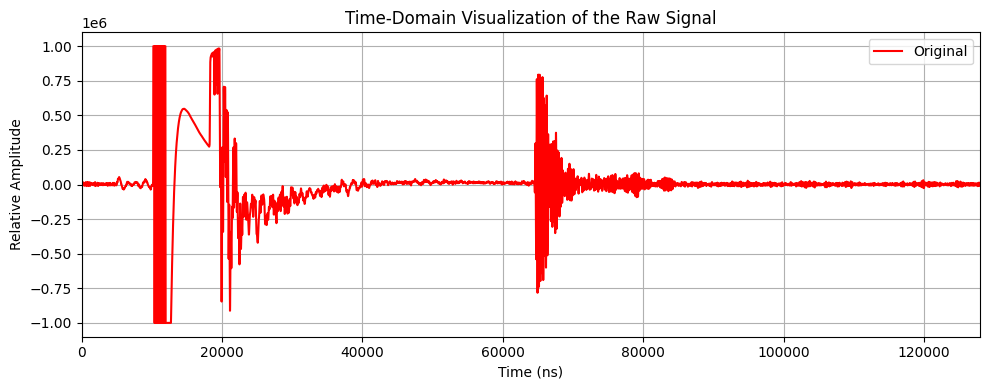
\includegraphics[width=0.75\linewidth]{raw_signal.png}
    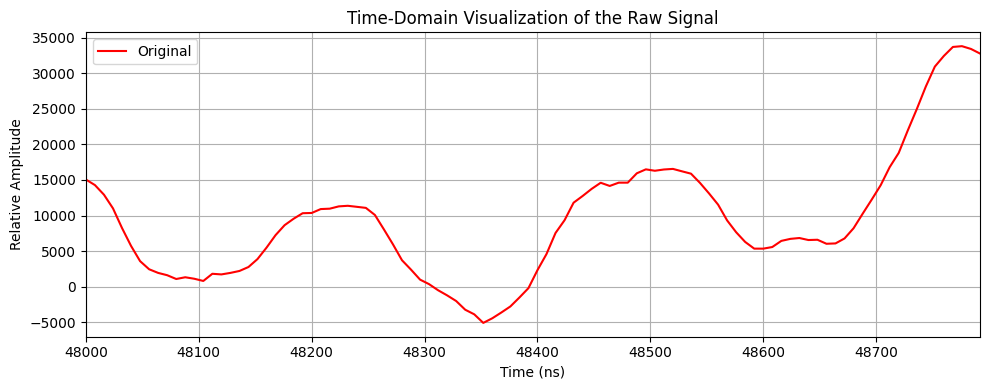
\includegraphics[width=0.75\linewidth]{rawsignal.png}

    \caption{Raw Signal}

    \label{fig:enter-label}
\end{figure}

\begin{figure}
    \centering
    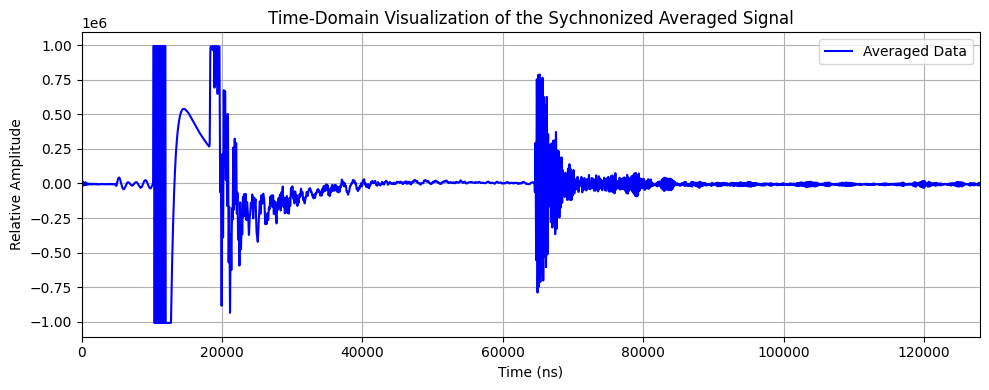
\includegraphics[width=0.75\linewidth]{time_synchonized.png}
    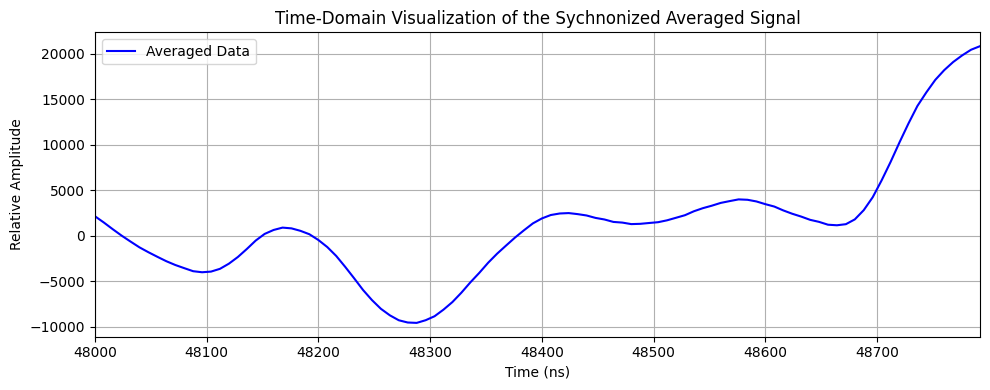
\includegraphics[width=0.75\linewidth]{timesynchonized.png}

    \caption{Time synchronized averaging of signal}
    \label{fig:enter-label}
\end{figure}


\begin{figure}[t]
    \centering
    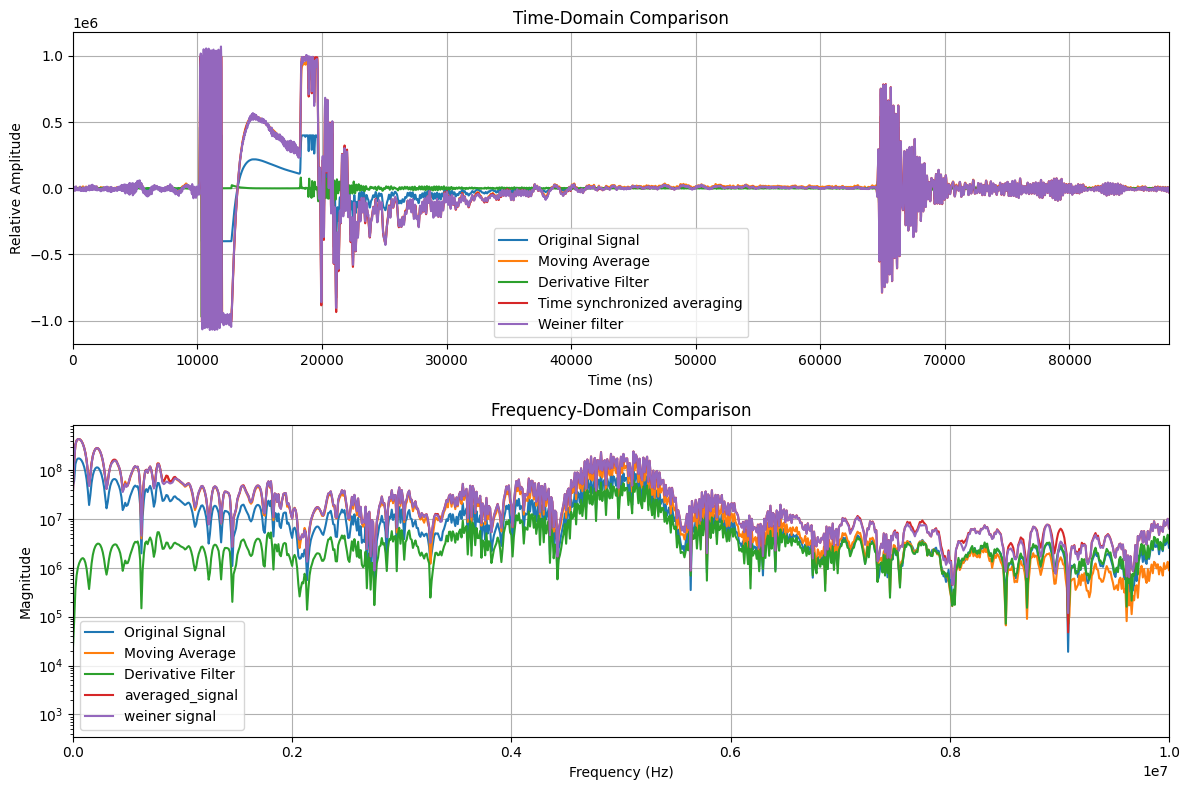
\includegraphics[width=0.75\linewidth]{comparision of signals.png}
    \caption{Comparison of various filtering techniques}
    \label{fig:enter-label}
\end{figure}

\section{Time-of-Flight and Velocity Estimation}
We found several key factors that affect signal behavior and the precision of sugar detection. These include: sugar concentration, liquid density, adiabatic compressibility, room and liquid temperature, ultrasonic frequency, air pressure, water pressure, acoustic impedance, air bubbles, vessel material and dimensions, sensor placement, signal-to-noise ratio, noise level, sensor sensitivity. \cite{citation5}\cite{citation6}
\vspace{1em}  % adds vertical space (~line break)


We performed the measurement at various temperatures, but at 45 degree Celsius, we observed damped signals, which introduced us to the effect of degassing \cite{citation9}, as mentioned the readings are highly affected by air bubbles and formation of them resulted in damping of the signal which was initially confused with attenuation. Although, attenuation was initially considered as a feature, but due to low sugar concentrations and limited density, we were not able to deduct any relationship.
\vspace{1em}  % adds vertical space (~line break)
 
The Time-of-Flight (ToF) is defined as the difference between the time when the signal is received and the time it was transmitted:

\begin{equation}
\Delta t = t_{\text{received}} - t_{\text{transmitted}}
\label{eq:tof}
\end{equation}

Using this ToF, the velocity \( v \) of the ultrasonic wave in the medium can be calculated using the known distance \( x \) between the transducer and the reflecting surface:

\begin{equation}
v = \frac{x}{t_2 - t_1} = \frac{x}{\Delta t}
\label{eq:velocity}
\end{equation}


\begin{figure}[t]
\centering
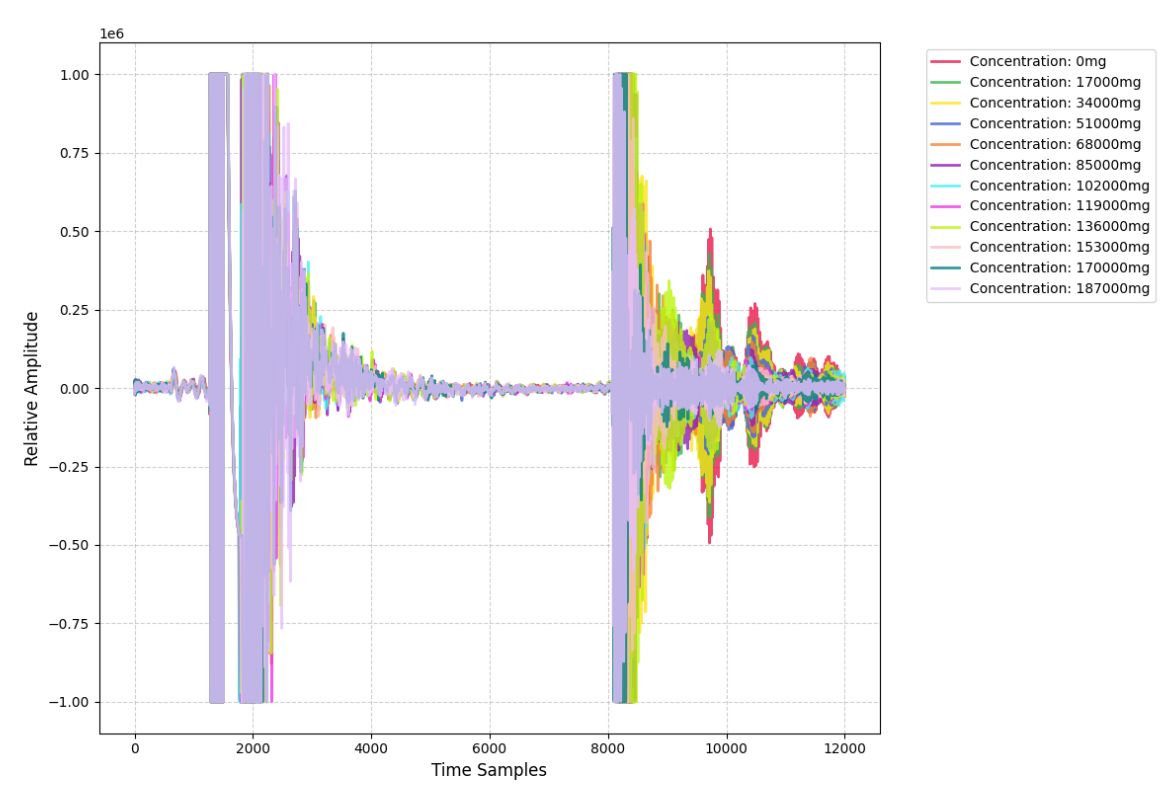
\includegraphics[width=0.75\textwidth]{overlaid.png}
\caption{Overlaid echoes from multiple measurements across increasing sugar concentrations.}
\label{fig:fig1}
\end{figure}
\vspace{1em}  % adds vertical space (~line break)


With the increasing sugar concentration, shifts in the amplitude, phase, and the arrival time of the echo become evident (Figure~\ref{fig:fig1}) . These subtle shifts form the baseline for further Time of Flight (TOF) and velocity calculation\cite{citation7}
\vspace{1em}  % adds vertical space (~line break)

Time-of-Flight (ToF) and the ultrasonic velocity ($v$) were evaluated using both zero-crossing detection method \cite{citation8} and peak-to-peak detection approach.

\subsubsection*{Peak to peak approach:} Leveraged Local maxima and minima in both transmitted and received signals using a prominence filter. Followed by the selection of strongest peak (with highest amplitude) from each signal. \cite{citation11}

The indices of the selected peaks in the transmitted and received signals are noted as \( t1_{\text{transmit}} \) and \( t2_{\text{receive}} \), respectively. The Time-of-Flight (ToF) is then calculated using the following equation:

\begin{equation}
\text{ToF (s)} = (t2_{\text{receive}} - t1_{\text{transmit}}) \times \frac{1}{f_s}
\label{eq:tof-discrete}
\end{equation}

where \( f_s \) is the sampling frequency (in Hz), and \( \frac{1}{f_s} \) is the time resolution of each sample.

\subsubsection*{Zero- Crossing approach:} In this method, the time-of-flight is estimated by identifying the first prominent zero-crossing in both the transmitted and received signals. A zero-crossing is defined as the point where the signal waveform crosses the zero-amplitude line, transitioning from positive to negative or vice versa.\cite{citation10}
\begin{figure}[t]
    \centering
    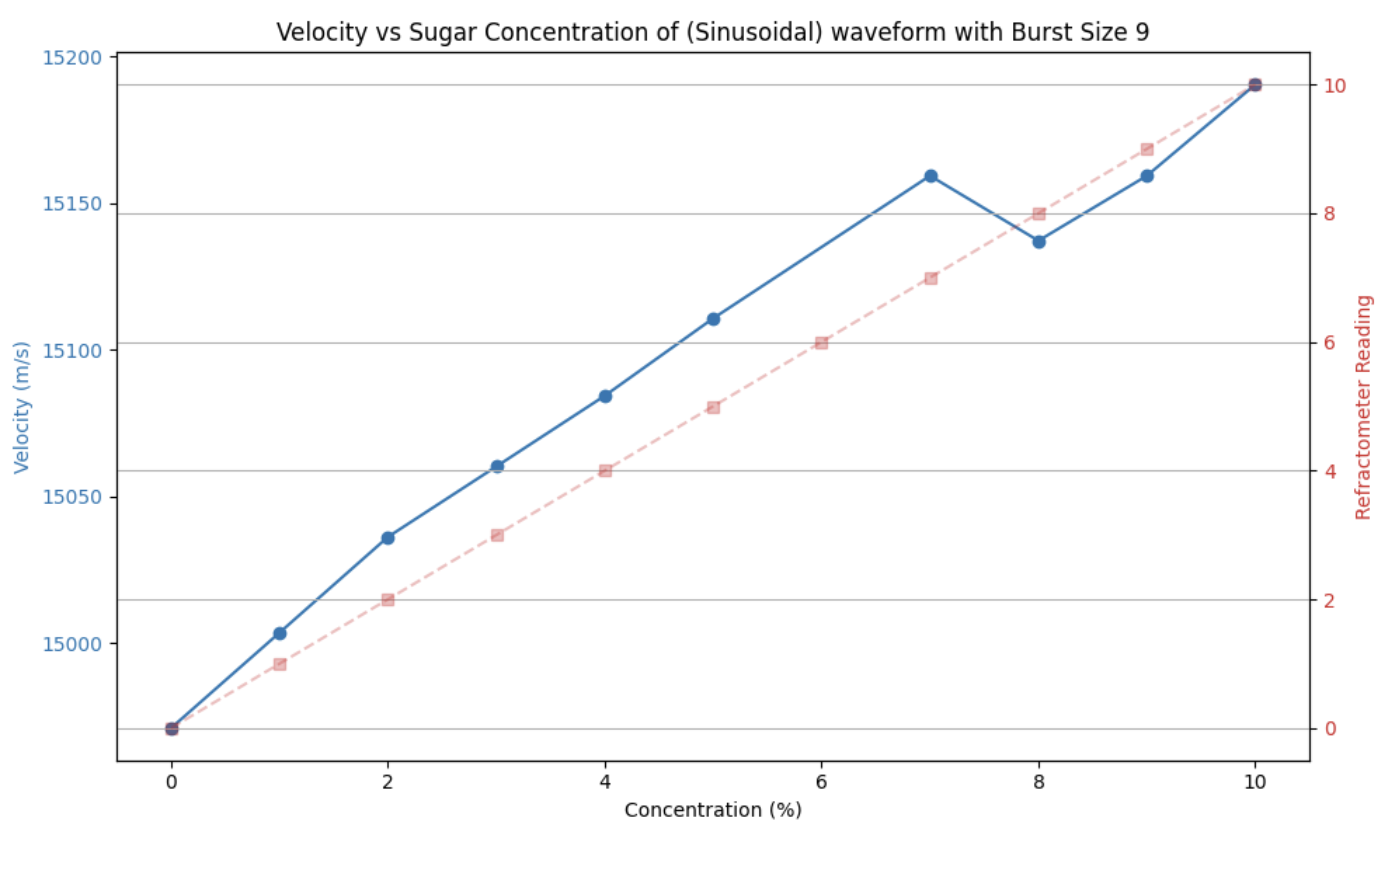
\includegraphics[width=0.75\linewidth]{peaktopeak.png}
        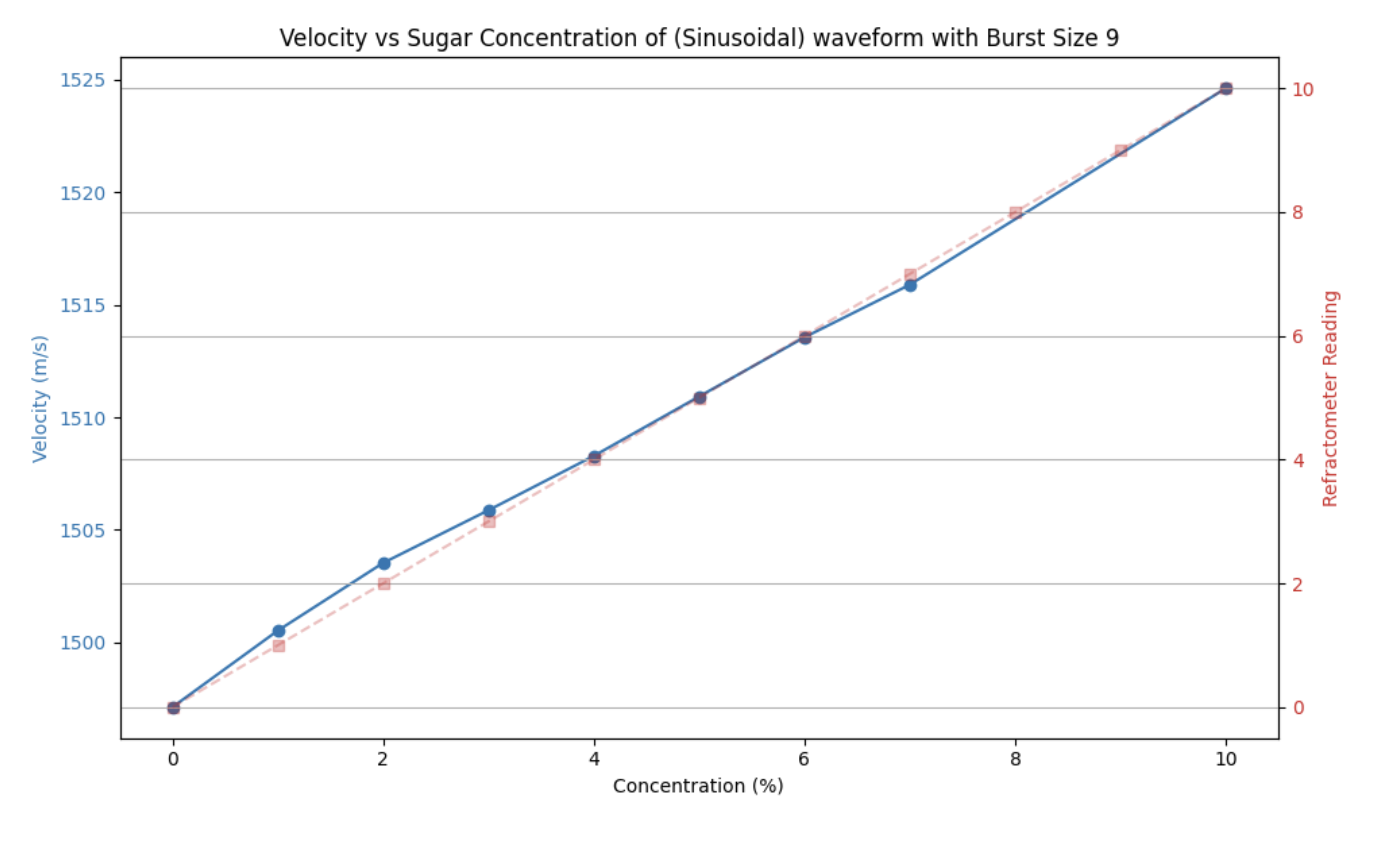
\includegraphics[width=0.75\linewidth]{zero__crossing.png}

    \caption{Peak to Peak Measurement and zero crossing approach respectively.}
    \end{figure}

%\begin{figure}
   % \centering
   % 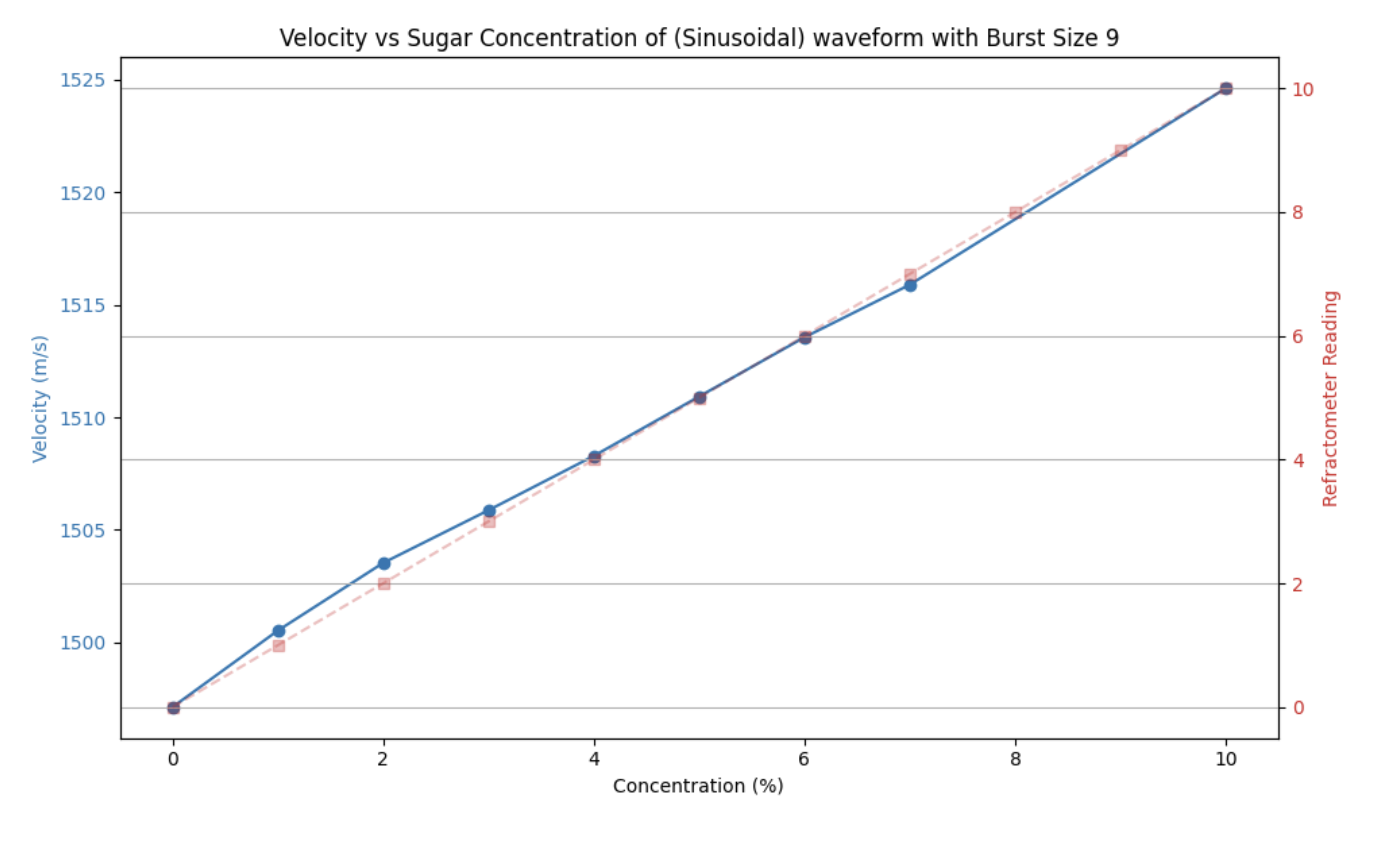
\includegraphics[width=0.75\linewidth]{zero__crossing.png}
  %  \caption{Zero-Crossing approach}
  %  \label{fig:enter-label}
%\end{figure}


Overall, the zero crossing detection method consistently performed better. On the other hand, the peak-to-peak approach proved to be more prone to artifacts and waveform distortions, making it less reliable for precise ToF calculation usually when signals are low in amplitude or highly attenuated.



\section{Results}

In this research, we realized that CMUT sensor can detect subtle sugar concentrations in liquids.The calculation of TOF and ultrasonic velocity with respect to increasing sugar concentrations resulted in a monotonic quasi-linear trend which can identify the measured sugar concentration in the range of 0 to 10\% for 1\% and even 0.1\% resolution which outperforms the state of the art.– see exemplary Figure~\ref{fig:fig2} and Figure~\ref{fig:fig3}.



\begin{figure}[t]
\centering
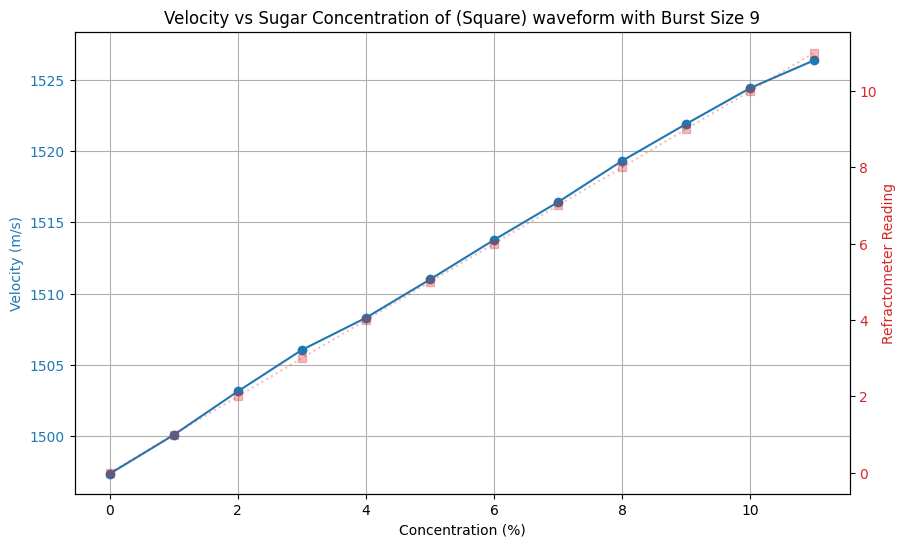
\includegraphics[width=0.7\textwidth]{Bild (1).png}
\caption{Ultrasonic velocity vs. sugar concentration (1\%-10\%) showing a clear monotonic trend}
\label{fig:fig2}
\end{figure}

\vspace{-10pt} % Reduces vertical space


\begin{figure}[t]
\centering
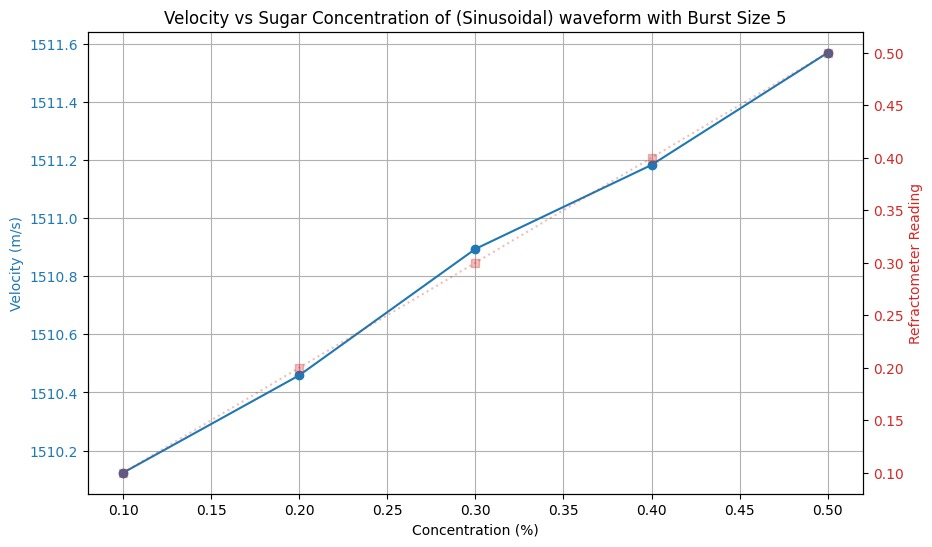
\includegraphics[width=0.7\textwidth]{lowconcentration.jpeg}
\caption{Detection of precise velocity shifts for low sugar concentrations (0.1\%-0.5\%)}
\label{fig:fig3}
\end{figure}

\section{Conclusion and Future Work}
The results in Figures~\ref{fig:fig2} and~\ref{fig:fig3} demonstrate the system’s sensitivity to both low and high sugar concentrations. Even in the low concentration range (0.1\%–0.5\%), the system was able to detect subtle changes in ultrasonic velocity, indicating a high resolution capability.

Preliminary studies focused on experimental data modeling have shown that the resolution and accuracy of sugar concentration estimation can be further improved to the ranges relevant to glucose detection in the human body.

While the current study demonstrates the suitability of using CMUT-based ultrasonic sensing for detecting low sugar concentrations in water, several areas remain open for further exploration:
\begin{itemize}
\item Frequency Domain Analysis for Velocity Calculation: Using Helmholtz equation and Neuman conditions.
\item Effect of Synthetic Blood as a Medium: Which could be synthesized using 40\& glycerin and 60\% water.
\item Predictive modeling for Sugar Concentration using various neural network models.
\end{itemize}

\begin{thebibliography}{8}
\bibitem{citation1}
Hossain MJ, Al-Mamun M, Islam MR. Diabetes mellitus, the fastest growing global public health concern: Early detection should be focused. Health Sci Rep. 2024 Mar 22;7(3):e2004. doi: 10.1002/hsr2.2004. PMID: 38524769; PMCID: PMC10958528. \url{https://pmc.ncbi.nlm.nih.gov/articles/PMC10958528/}

\bibitem{citation2}
Mayo Clinic Staff: Blood sugar testing: Why, when and how \url{https://www.mayoclinic.org/diseases-conditions/diabetes/in-depth/blood-sugar/art-20046628}

\bibitem{citation3}
Fraunhofer IPMS: Capacitive Micromachined Ultrasonic Transducer (CMUT). \url{https://www.ipms.fraunhofer.de/en/Components-and-Systems/Components-and-Systems-Sensors/Ultrasonic-Sensors/Capacitive-micromachined-ultrasonic-transducer-CMUT.html}

\bibitem{citation4}
Calculla: Acoustic impedance of various materials table \url{https://calculla.com/acoustic_impedance_of_materials}

\bibitem{citation5}
Hoche S, Hussein MA, Becker T. Density, ultrasound velocity, acoustic impedance, reflection and absorption coefficient determination of liquids via multiple reflection method. Ultrasonics. 2015 Mar;57:65-71. doi: 10.1016/j.ultras.2014.10.017. Epub 2014 Oct 30. PMID: 25465962.\url{https://pubmed.ncbi.nlm.nih.gov/25465962/}

\bibitem{citation6}
Kazys R, Rekuviene R, Sliteris R, Mazeika L, Zukauskas E. Ultrasonic technique for monitoring of liquid density variations. Rev Sci Instrum. 2015 Jan;86(1):015003. doi: 10.1063/1.4905570. PMID: 25638115.
\url{https://pubmed.ncbi.nlm.nih.gov/25638115/}

\bibitem{citation7}
L. Shi, L. Jia, C. Liu, C. Sun, S. Liu and G. Wu, "A Miniaturized Ultrasonic Sugar Concentration Detection System Based on Piezoelectric Micromachined Ultrasonic Transducers," in IEEE Transactions on Instrumentation and Measurement, vol. 71, pp. 1-9, 2022, Art no. 7503509, doi: 10.1109/TIM.2022.3185650.
\url{https://ieeexplore.ieee.org/abstract/document/9804879}

\bibitem{citation8}
Sunol, Francesc \& Ochoa Guerrero, Diego Alejandro \& Garcia, Jose. (2018). High-Precision Time-of-Flight Determination Algorithm for Ultrasonic Flow Measurement. IEEE Transactions on Instrumentation and Measurement. PP. 1-9. 10.1109/TIM.2018.2869263. \url{https://www.researchgate.net/publication/327850361_High-Precision_Time-of-Flight_Determination_Algorithm_for_Ultrasonic_Flow_Measurement}

\bibitem{citation9}

Degassing and Temperature Effects on the Formation of Nanobubbles at the Mica/Water Interface
Xue H. Zhang, Xiao D. Zhang, Shi T. Lou, Zhi X. Zhang, Jie L. Sun, and Jun Hu
Langmuir 2004 20 (9), 3813-3815
DOI: 10.1021/la0364542
\url{https://pubs.acs.org/action/showCitFormats?doi=10.1021%2Fla0364542&include=cit&format=ris&direct=true&downloadFileName=la0364542&href=/doi/10.1021/la0364542}

\bibitem{citation10}

Zehua Fang, Rui Su, Liang Hu, Xin Fu,
A simple and easy-implemented time-of-flight determination method for liquid ultrasonic flow meters based on ultrasonic signal onset detection and multiple-zero-crossing technique,
Measurement,
Volume 168,
2021,
108398,
ISSN 0263-2241,
https://doi.org/10.1016/j.measurement.2020.108398.
\url{https://www.sciencedirect.com/science/article/pii/S0263224120309337}


\bibitem{citation11}
Ying Zheng, Di Tian, Ke Liu, Zemin Bao, Peizhi Wang, Chunling Qiu, Dunyi Liu, Runlong Fan,
Peak detection of TOF-SIMS using continuous wavelet transform and curve fitting,
International Journal of Mass Spectrometry,
Volume 428,
2018,
Pages 43-48,
ISSN 1387-3806,
https://doi.org/10.1016/j.ijms.2018.03.001.
\url{https://www.sciencedirect.com/science/article/pii/S1387380618300071}


\end{thebibliography}
\end{document}
